\documentclass[a4paper,12pt]{article}
\usepackage[utf8]{vietnam}
\usepackage{amsmath}
\usepackage{algorithm}
\usepackage{algpseudocode}
\usepackage{graphicx}

\begin{document}

\section{Thuật toán tăng cường dữ liệu thích ứng}

\subsection{Cơ sở lý thuyết}
Trong nhận diện biểu cảm khuôn mặt (FER) dưới điều kiện ánh sáng yếu, chất lượng ảnh thường bị suy giảm do độ sáng thấp. Các kỹ thuật tăng cường dữ liệu cố định như \textit{histogram equalization} hoặc \textit{gamma correction} không tối ưu vì chúng áp dụng đồng nhất cho mọi ảnh. Thuật toán \textbf{tăng cường dữ liệu thích ứng} được thiết kế để phân tích mức độ ánh sáng của từng ảnh và áp dụng kỹ thuật tăng cường phù hợp.

Thuật toán dựa trên các cơ sở lý thuyết sau:
\begin{itemize}
    \item \textbf{Phân tích độ sáng}: Độ sáng trung bình (\( \mu \)) của ảnh grayscale được sử dụng để đánh giá mức độ ánh sáng yếu.
    \item \textbf{Kỹ thuật tăng cường}:
    \begin{itemize}
        \item \textit{Gamma correction}: \( I_{\text{out}} = I_{\text{in}}^{\gamma} \), với \( \gamma < 1 \) để tăng độ sáng.
        \item \textit{Histogram equalization}: Tăng độ tương phản bằng cách phân bố lại giá trị pixel.
        \item \textit{Contrast stretching}: Kéo dãn khoảng giá trị pixel.
    \end{itemize}
    \item \textbf{Tính thích ứng}: Dựa trên \( \mu \) và các ngưỡng \( T_1, T_2 \), thuật toán chọn kỹ thuật tăng cường phù hợp.
\end{itemize}

\subsection{Mô tả thuật toán}
Thuật toán được trình bày như sau:

\begin{algorithm}
\caption{Tăng cường dữ liệu thích ứng}
\begin{algorithmic}[1]
\Require Ảnh đầu vào \( I \), ngưỡng \( T_1, T_2 \), giá trị gamma \( \gamma_{\text{low}}, \gamma_{\text{mid}} \)
\Ensure Ảnh tăng cường \( I_{\text{out}} \)
\State Chuyển \( I \) sang grayscale để tính độ sáng trung bình \( \mu \)
\If{\( \mu < T_1 \)}
    \State Áp dụng \textit{gamma correction} với \( \gamma = \gamma_{\text{low}} \)
    \State \( I_{\text{out}} \gets \text{GammaCorrection}(I, \gamma_{\text{low}}) \)
\ElsIf{\( T_1 \leq \mu < T_2 \)}
    \State Áp dụng \textit{gamma correction} với \( \gamma = \gamma_{\text{mid}} \)
    \State \( I_{\text{out}} \gets \text{GammaCorrection}(I, \gamma_{\text{mid}}) \)
\Else
    \State Áp dụng \textit{contrast stretching}
    \State \( I_{\text{out}} \gets \text{ContrastStretching}(I) \)
\EndIf
\State \Return \( I_{\text{out}} \)
\end{algorithmic}
\end{algorithm}

\subsection{Ưu điểm}
\begin{itemize}
    \item \textbf{Tính thích ứng}: Tùy chỉnh tăng cường dựa trên đặc trưng ánh sáng của từng ảnh.
    \item \textbf{Đơn giản}: Dễ triển khai, phù hợp với mô hình nhẹ như MobileNetV3.
    \item \textbf{Hiệu quả}: Cải thiện chất lượng ảnh, hỗ trợ nhận diện biểu cảm tốt hơn.
\end{itemize}

\subsection{Khuyết điểm}
\begin{itemize}
    \item \textbf{Phụ thuộc ngưỡng}: Hiệu quả phụ thuộc vào việc chọn \( T_1, T_2 \).
    \item \textbf{Hạn chế với ánh sáng không đồng đều}: Không xử lý tốt vùng tối cục bộ.
    \item \textbf{Không xử lý nhiễu}: Có thể cần thêm bước giảm nhiễu.
\end{itemize}

\subsection{Triển khai thuật toán}
Thuật toán được triển khai bằng Python với các thư viện OpenCV và NumPy. Dưới đây là một ví dụ minh họa:

\begin{figure}[h]
    \centering
    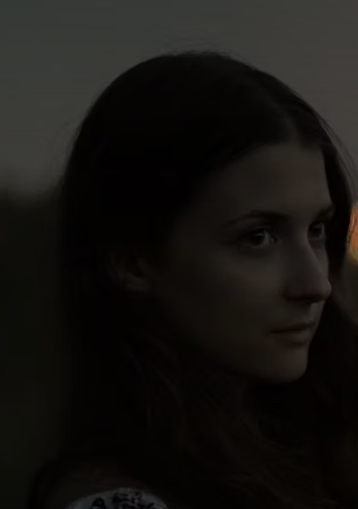
\includegraphics[width=0.8\textwidth]{dark_image.png}
    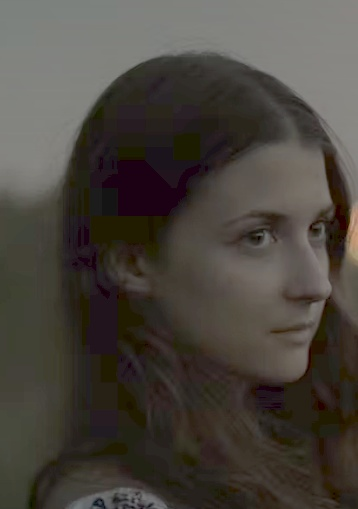
\includegraphics[width=0.8\textwidth]{gamma_corrected.png}
    \caption{Kết quả tăng cường dữ liệu thích ứng trên ảnh ánh sáng yếu.}
\end{figure}

\end{document}